\section{Limits}

Limits are important in calculus since we need very small quantities to effectively study change. Yeah, that's pretty vague, but hopefully it'll clear up in a few pages.

We study limits for many reasons. One of them is to study functions at points where they are only ``close'' to being defined. For example, the function $f$ given by $f(x)=\frac{x(x+1)}{x}$ is not defined at $0$, but looks like the line $x+1$ everywhere else.

\subsection{Intuitive Limits}

The intuitive idea of a \textbf{limit} is to examine what the output of a function does as the input moves close to a specific value. Since the functions we care about take real numbers as inputs, there are two ways you can approach a number on the real line (from the left and from the right). We will talk about left- and right-sided limits.

Before getting into the actual definition, we'll start intuitively. If a function is     ``continuous''\footnote{I put this word in quotes because I haven't defined it yet, but you should have an intuitive idea of what this means: being able to draw it without lifting your pencil. Just wait for a few pages.} and is defined at $a$, then as $x$ moves closer to $a$, $f(x)$ moves closer to $f(a)$, so the limit of $f$ as $x$ approaches $a$ is $f(a)$.


Let's get a little more general: suppose a function $f$ is defined on open intervals on either side of $a$.

If $f$ is defined on an interval to the \textit{left} of $a$ and the values of $f(x)$ approach $L$ as $x$ approaches $a$ from the \textit{left}, we say that the ``\textbf{left-sided limit of $f$ as $x$ approaches $a$} is $L$'' and we write $$\lim_{x\to a^-}f(x)=L.$$
If $f$ is defined on an interval to the \textit{right} of $a$ and the values of $f(x)$ approach $L$ as $x$ approaches $a$ from the \textit{right}, we say that the \textbf{right-sided limit of $f$ as $x$ approaches $a$} is $L$'' and we write
$$\lim_{x\to a^+}f(x)=L.$$
If the right and left sided limits match, then we say that the \textbf{limit of $f$ as $x$ approaches $a$ is $L$} and write $$\lim_{x\to a}f(x)=L.$$

\noindent Note: $f$ need not be defined at $a$ to find the limit of $f$ as $x$ approaches $a$.

\vspace{1em}

One can compute $f(x)$ for values of $x$ that get closer and closer to either side of $a$. If the values approach $L$, then you have good reason to believe that $L$ is the (right- and/or left-sided) limit.

\begin{center}
\begin{tabular}{@{}ll@{}}
\toprule[0.4mm]
   $x$        & $f(x)$        \\
\midrule
   $a-0.1$    & $f(a-0.1)$    \\
   $a-0.01$   & $f(a-0.01)$   \\
   $a-0.001$  & $f(a-0.001)$  \\
   $a-0.0001$ & $f(a-0.0001)$ \\
\midrule
   $a+0.0001$ & $f(a+0.0001)$ \\
   $a+0.001$  & $f(a+0.001)$  \\
   $a+0.01$   & $f(a+0.01)$   \\
   $a+0.1$    & $f(a+0.1)$    \\
\bottomrule[0.4mm]
\end{tabular}
\end{center}
Such calculations, however, cannot prove that a function limits to a specific value.

\subsection{Infinite Limits}

We can extend the idea of limits outside of the real numbers to include positive and negative infinity in place of both $a$ and $L$.
\begin{itemize}
\item If $f(x)$ grows without bound as $x$ approaches $a$ from the left, then we write $$\lim_{x\to a^-}f(x)=\infty.$$
(Similarly for $x$ approaching $a$ from the right, and also if $f(x)$ becomes increasingly negative without bound).
\item We denote the value (if such a value exists) that $f(x)$ approaches as $x$ approaches $\infty$ as $$\lim_{x\to\infty} f(x).$$
(Similarly if $x$ approaches $-\infty$).
\end{itemize}



\subsection{Optional: The $\varepsilon-\delta$ Definition}

You may be dissatisfied with the intuitive approach to limits, so we can make the definition more rigorous. The main idea that needs to be captured by a formal definition is \textit{arbitrary precision}. That is, we need a way to say formally that ``$f(x)$ approaches $L$ as $x$ approaches $a$.''

By controlling the input $x$, we must be able to make the distance $|f(x)-L|$ between the output $f(x)$ and $L$ to be as small as we want (``arbitrarily small''). In other words, if $\varepsilon>0$ is any small positive number, we must be able to ensure (by controlling $x$) that $|f(x)-L| < \varepsilon$. To control $x$, we can make the distance $|x-a|$ between $x$ and $a$ smaller than some positive number $\delta > 0$ (that may depend on $\varepsilon$).

Now we're ready for the real ``$\varepsilon-\delta$'' definition of a limit: we say that \textbf{$L$ is the limit of $f$ as $x$ approaches $a$} if
$$\text{for all } \varepsilon > 0, \text{ there is some } \delta > 0, \text{ such that } |x - a| < \delta \implies |f(x) - L| <\varepsilon.$$

Read that last line a few times, because statements with multiple quantifiers can be tricky!

\begin{figure}[h!]
\centering
\fbox{
\tikzset{every picture/.style={line width=0.75pt}}
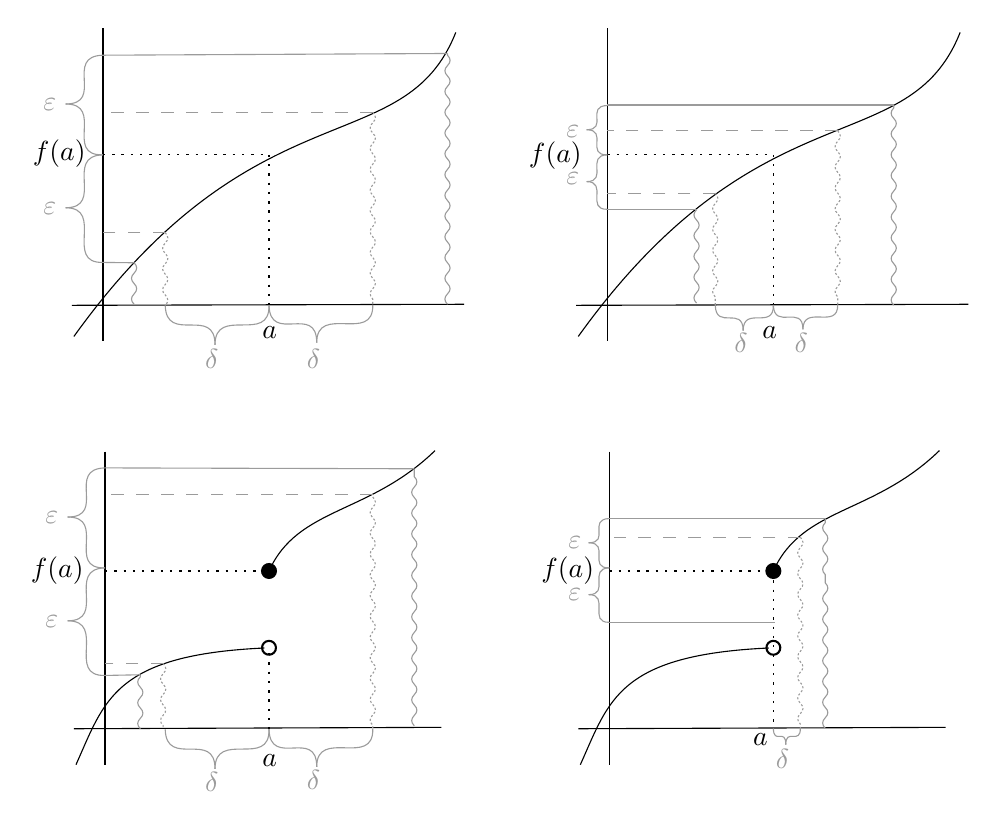
\begin{tikzpicture}[x=0.75pt,y=0.75pt,yscale=-1,xscale=1]
%uncomment if require: \path (0,428); %set diagram left start at 0, and has height of 428

%Straight Lines [id:da2730924968926851]
\draw    (71,155) -- (260,154.5) ;
%Straight Lines [id:da38663844155403493]
\draw    (86,21.5) -- (86,172.33) ;
%Curve Lines [id:da5832897062677318]
\draw    (72,170) .. controls (160,47.5) and (231,86.5) .. (256,23.5) ;
%Curve Lines [id:da15926967534570857]
\draw    (73,376.33) .. controls (86.86,345.64) and (90.92,323.45) .. (163.77,320.1) ;
\draw [shift={(166,320)}, rotate = 357.71] [color={rgb, 255:red, 0; green, 0; blue, 0 }  ][line width=0.75]      (0, 0) circle [x radius= 3.35, y radius= 3.35]   ;
%Curve Lines [id:da573129079856388]
\draw    (166,283) .. controls (180,252) and (214,256) .. (246,225) ;
\draw [shift={(166,283)}, rotate = 294.3] [color={rgb, 255:red, 0; green, 0; blue, 0 }  ][fill={rgb, 255:red, 0; green, 0; blue, 0 }  ][line width=0.75]      (0, 0) circle [x radius= 3.35, y radius= 3.35]   ;
%Straight Lines [id:da06544192635535961]
\draw  [dash pattern={on 0.84pt off 2.51pt}]  (166,82.5) -- (166,154.92) ;
%Straight Lines [id:da8462520068785757]
\draw  [dash pattern={on 0.84pt off 2.51pt}]  (86,82.5) -- (166,82.5) ;
%Straight Lines [id:da8033956316212987]
\draw [color={rgb, 255:red, 155; green, 155; blue, 155 }  ,draw opacity=1 ]   (86,34.5) -- (252,33.67) ;
%Straight Lines [id:da9058328806059841]
\draw [color={rgb, 255:red, 155; green, 155; blue, 155 }  ,draw opacity=1 ]   (86,134.33) -- (101,134.5) ;
%Straight Lines [id:da7683874289412185]
\draw    (72,359) -- (249,358.33) ;
%Straight Lines [id:da21021021460529377]
\draw    (87,225.5) -- (87,376.33) ;
%Straight Lines [id:da5263630709862186]
\draw  [dash pattern={on 0.84pt off 2.51pt}]  (166,322.58) -- (166,359.25) ;
%Straight Lines [id:da2255352189878881]
\draw  [dash pattern={on 0.84pt off 2.51pt}]  (87,283) -- (166,283) ;
%Straight Lines [id:da12241776303117424]
\draw [color={rgb, 255:red, 155; green, 155; blue, 155 }  ,draw opacity=1 ]   (87,233.33) -- (236,233.75) ;
%Straight Lines [id:da6551551228954233]
\draw [color={rgb, 255:red, 155; green, 155; blue, 155 }  ,draw opacity=1 ]   (87,333.33) -- (104,333) ;
%Straight Lines [id:da3470258564776276]
\draw [color={rgb, 255:red, 155; green, 155; blue, 155 }  ,draw opacity=1 ] [dash pattern={on 0.75pt off 0.75pt}]  (116,120) .. controls (117.67,121.67) and (117.67,123.33) .. (116,125) .. controls (114.33,126.67) and (114.33,128.33) .. (116,130) .. controls (117.67,131.67) and (117.67,133.33) .. (116,135) .. controls (114.33,136.67) and (114.33,138.33) .. (116,140) .. controls (117.67,141.67) and (117.67,143.33) .. (116,145) .. controls (114.33,146.67) and (114.33,148.33) .. (116,150) .. controls (117.67,151.67) and (117.67,153.33) .. (116,155) -- (116,155) ;
%Straight Lines [id:da2371091562631653]
\draw [color={rgb, 255:red, 155; green, 155; blue, 155 }  ,draw opacity=1 ] [dash pattern={on 0.75pt off 0.75pt}]  (216,62) .. controls (217.67,63.67) and (217.67,65.33) .. (216,67) .. controls (214.33,68.67) and (214.33,70.33) .. (216,72) .. controls (217.67,73.67) and (217.67,75.33) .. (216,77) .. controls (214.33,78.67) and (214.33,80.33) .. (216,82) .. controls (217.67,83.67) and (217.67,85.33) .. (216,87) .. controls (214.33,88.67) and (214.33,90.33) .. (216,92) .. controls (217.67,93.67) and (217.67,95.33) .. (216,97) .. controls (214.33,98.67) and (214.33,100.33) .. (216,102) .. controls (217.67,103.67) and (217.67,105.33) .. (216,107) .. controls (214.33,108.67) and (214.33,110.33) .. (216,112) .. controls (217.67,113.67) and (217.67,115.33) .. (216,117) .. controls (214.33,118.67) and (214.33,120.33) .. (216,122) .. controls (217.67,123.67) and (217.67,125.33) .. (216,127) .. controls (214.33,128.67) and (214.33,130.33) .. (216,132) .. controls (217.67,133.67) and (217.67,135.33) .. (216,137) .. controls (214.33,138.67) and (214.33,140.33) .. (216,142) .. controls (217.67,143.67) and (217.67,145.33) .. (216,147) .. controls (214.33,148.67) and (214.33,150.33) .. (216,152) -- (216,154.71) -- (216,154.71) ;
%Straight Lines [id:da47940446384008517]
\draw [color={rgb, 255:red, 155; green, 155; blue, 155 }  ,draw opacity=1 ] [dash pattern={on 4.5pt off 4.5pt}]  (116,120) -- (86,120) ;
%Straight Lines [id:da2718218581855085]
\draw [color={rgb, 255:red, 155; green, 155; blue, 155 }  ,draw opacity=1 ] [dash pattern={on 4.5pt off 4.5pt}]  (216,62) -- (86,62) ;
%Curve Lines [id:da7867325499156288]
\draw [color={rgb, 255:red, 155; green, 155; blue, 155 }  ,draw opacity=1 ]   (68,58) .. controls (87,58) and (67,35) .. (86,34.5) ;
%Curve Lines [id:da8389021578247982]
\draw [color={rgb, 255:red, 155; green, 155; blue, 155 }  ,draw opacity=1 ]   (68,58) .. controls (87,58) and (67,83) .. (86,82.5) ;
%Curve Lines [id:da6940267896547274]
\draw [color={rgb, 255:red, 155; green, 155; blue, 155 }  ,draw opacity=1 ]   (68,108) .. controls (87,108) and (67,83) .. (86,82.5) ;
%Curve Lines [id:da9368251006708403]
\draw [color={rgb, 255:red, 155; green, 155; blue, 155 }  ,draw opacity=1 ]   (68,108) .. controls (87,108) and (67,134.83) .. (86,134.33) ;
%Curve Lines [id:da7416463958304471]
\draw [color={rgb, 255:red, 155; green, 155; blue, 155 }  ,draw opacity=1 ]   (139.99,174) .. controls (140,155) and (116.5,174) .. (116,155) ;
%Curve Lines [id:da0946019041451891]
\draw [color={rgb, 255:red, 155; green, 155; blue, 155 }  ,draw opacity=1 ]   (139.99,174) .. controls (140,155) and (166.5,173.92) .. (166,154.92) ;
%Curve Lines [id:da8479225025412045]
\draw [color={rgb, 255:red, 155; green, 155; blue, 155 }  ,draw opacity=1 ]   (188.99,173) .. controls (189,154) and (166.5,173.92) .. (166,154.92) ;
%Curve Lines [id:da5287374586288269]
\draw [color={rgb, 255:red, 155; green, 155; blue, 155 }  ,draw opacity=1 ]   (188.99,173) .. controls (189,154) and (216.5,173.71) .. (216,154.71) ;
%Straight Lines [id:da5763369512697336]
\draw [color={rgb, 255:red, 155; green, 155; blue, 155 }  ,draw opacity=1 ]   (101,154.5) .. controls (99.33,152.83) and (99.33,151.17) .. (101,149.5) .. controls (102.67,147.83) and (102.67,146.17) .. (101,144.5) .. controls (99.33,142.83) and (99.33,141.17) .. (101,139.5) .. controls (102.67,137.83) and (102.67,136.17) .. (101,134.5) -- (101,134.5) ;
%Straight Lines [id:da9925497456851824]
\draw [color={rgb, 255:red, 155; green, 155; blue, 155 }  ,draw opacity=1 ]   (252,154.5) .. controls (250.33,152.83) and (250.33,151.17) .. (252,149.5) .. controls (253.67,147.83) and (253.67,146.17) .. (252,144.5) .. controls (250.33,142.83) and (250.33,141.17) .. (252,139.5) .. controls (253.67,137.83) and (253.67,136.17) .. (252,134.5) .. controls (250.33,132.83) and (250.33,131.17) .. (252,129.5) .. controls (253.67,127.83) and (253.67,126.17) .. (252,124.5) .. controls (250.33,122.83) and (250.33,121.17) .. (252,119.5) .. controls (253.67,117.83) and (253.67,116.17) .. (252,114.5) .. controls (250.33,112.83) and (250.33,111.17) .. (252,109.5) .. controls (253.67,107.83) and (253.67,106.17) .. (252,104.5) .. controls (250.33,102.83) and (250.33,101.17) .. (252,99.5) .. controls (253.67,97.83) and (253.67,96.17) .. (252,94.5) .. controls (250.33,92.83) and (250.33,91.17) .. (252,89.5) .. controls (253.67,87.83) and (253.67,86.17) .. (252,84.5) .. controls (250.33,82.83) and (250.33,81.17) .. (252,79.5) .. controls (253.67,77.83) and (253.67,76.17) .. (252,74.5) .. controls (250.33,72.83) and (250.33,71.17) .. (252,69.5) .. controls (253.67,67.83) and (253.67,66.17) .. (252,64.5) .. controls (250.33,62.83) and (250.33,61.17) .. (252,59.5) .. controls (253.67,57.83) and (253.67,56.17) .. (252,54.5) .. controls (250.33,52.83) and (250.33,51.17) .. (252,49.5) .. controls (253.67,47.83) and (253.67,46.17) .. (252,44.5) .. controls (250.33,42.83) and (250.33,41.17) .. (252,39.5) .. controls (253.67,37.83) and (253.67,36.17) .. (252,34.5) -- (252,33.67) -- (252,33.67) ;
%Curve Lines [id:da7131476230234577]
\draw [color={rgb, 255:red, 155; green, 155; blue, 155 }  ,draw opacity=1 ]   (69,257) .. controls (88,257) and (68,233.83) .. (87,233.33) ;
%Curve Lines [id:da5212410455410692]
\draw [color={rgb, 255:red, 155; green, 155; blue, 155 }  ,draw opacity=1 ]   (69,257) .. controls (88,257) and (68,282) .. (87,281.5) ;
%Curve Lines [id:da8037674418363849]
\draw [color={rgb, 255:red, 155; green, 155; blue, 155 }  ,draw opacity=1 ]   (69,307) .. controls (88,307) and (68,282) .. (87,281.5) ;
%Curve Lines [id:da3061502012065347]
\draw [color={rgb, 255:red, 155; green, 155; blue, 155 }  ,draw opacity=1 ]   (69,307) .. controls (88,307) and (68,333.83) .. (87,333.33) ;
%Curve Lines [id:da838846723146208]
\draw [color={rgb, 255:red, 155; green, 155; blue, 155 }  ,draw opacity=1 ]   (139.99,378.34) .. controls (140,359.34) and (116.5,378.33) .. (116,359.33) ;
%Curve Lines [id:da45926415056497105]
\draw [color={rgb, 255:red, 155; green, 155; blue, 155 }  ,draw opacity=1 ]   (139.99,378.34) .. controls (140,359.34) and (166.5,378.25) .. (166,359.25) ;
%Curve Lines [id:da1812164249288335]
\draw [color={rgb, 255:red, 155; green, 155; blue, 155 }  ,draw opacity=1 ]   (188.99,377.34) .. controls (189,358.34) and (166.5,378.25) .. (166,359.25) ;
%Curve Lines [id:da5310165714599331]
\draw [color={rgb, 255:red, 155; green, 155; blue, 155 }  ,draw opacity=1 ]   (188.99,377.34) .. controls (189,358.34) and (216.5,378.04) .. (216,359.04) ;
%Straight Lines [id:da1373743464903565]
\draw [color={rgb, 255:red, 155; green, 155; blue, 155 }  ,draw opacity=1 ] [dash pattern={on 0.75pt off 0.75pt}]  (115,327.5) .. controls (116.67,329.17) and (116.67,330.83) .. (115,332.5) .. controls (113.33,334.17) and (113.33,335.83) .. (115,337.5) .. controls (116.67,339.17) and (116.67,340.83) .. (115,342.5) .. controls (113.33,344.17) and (113.33,345.83) .. (115,347.5) .. controls (116.67,349.17) and (116.67,350.83) .. (115,352.5) .. controls (113.33,354.17) and (113.33,355.83) .. (115,357.5) -- (115,359) -- (115,359) ;
%Straight Lines [id:da30273639101181327]
\draw [color={rgb, 255:red, 155; green, 155; blue, 155 }  ,draw opacity=1 ] [dash pattern={on 0.75pt off 0.75pt}]  (216,247.33) .. controls (217.67,249) and (217.67,250.66) .. (216,252.33) .. controls (214.33,254) and (214.33,255.66) .. (216,257.33) .. controls (217.67,259) and (217.67,260.66) .. (216,262.33) .. controls (214.33,264) and (214.33,265.66) .. (216,267.33) .. controls (217.67,269) and (217.67,270.66) .. (216,272.33) .. controls (214.33,274) and (214.33,275.66) .. (216,277.33) .. controls (217.67,279) and (217.67,280.66) .. (216,282.33) .. controls (214.33,284) and (214.33,285.66) .. (216,287.33) .. controls (217.67,289) and (217.67,290.66) .. (216,292.33) .. controls (214.33,294) and (214.33,295.66) .. (216,297.33) .. controls (217.67,299) and (217.67,300.66) .. (216,302.33) .. controls (214.33,304) and (214.33,305.66) .. (216,307.33) .. controls (217.67,309) and (217.67,310.66) .. (216,312.33) .. controls (214.33,314) and (214.33,315.66) .. (216,317.33) .. controls (217.67,319) and (217.67,320.66) .. (216,322.33) .. controls (214.33,324) and (214.33,325.66) .. (216,327.33) .. controls (217.67,329) and (217.67,330.66) .. (216,332.33) .. controls (214.33,334) and (214.33,335.66) .. (216,337.33) .. controls (217.67,339) and (217.67,340.66) .. (216,342.33) .. controls (214.33,344) and (214.33,345.66) .. (216,347.33) .. controls (217.67,349) and (217.67,350.66) .. (216,352.33) .. controls (214.33,354) and (214.33,355.66) .. (216,357.33) -- (216,359.04) -- (216,359.04) ;
%Straight Lines [id:da6690760580285089]
\draw [color={rgb, 255:red, 155; green, 155; blue, 155 }  ,draw opacity=1 ] [dash pattern={on 4.5pt off 4.5pt}]  (115,327.5) -- (87,327.5) ;
%Straight Lines [id:da023392902319420816]
\draw [color={rgb, 255:red, 155; green, 155; blue, 155 }  ,draw opacity=1 ] [dash pattern={on 4.5pt off 4.5pt}]  (216,246) -- (87,246) ;
%Straight Lines [id:da7002803226646901]
\draw [color={rgb, 255:red, 155; green, 155; blue, 155 }  ,draw opacity=1 ]   (104,359) .. controls (102.33,357.33) and (102.33,355.67) .. (104,354) .. controls (105.67,352.33) and (105.67,350.67) .. (104,349) .. controls (102.33,347.33) and (102.33,345.67) .. (104,344) .. controls (105.67,342.33) and (105.67,340.67) .. (104,339) .. controls (102.33,337.33) and (102.33,335.67) .. (104,334) -- (104,333) -- (104,333) ;
%Straight Lines [id:da5440309336359443]
\draw [color={rgb, 255:red, 155; green, 155; blue, 155 }  ,draw opacity=1 ]   (236,357.58) .. controls (234.33,355.91) and (234.33,354.25) .. (236,352.58) .. controls (237.67,350.91) and (237.67,349.25) .. (236,347.58) .. controls (234.33,345.91) and (234.33,344.25) .. (236,342.58) .. controls (237.67,340.91) and (237.67,339.25) .. (236,337.58) .. controls (234.33,335.91) and (234.33,334.25) .. (236,332.58) .. controls (237.67,330.91) and (237.67,329.25) .. (236,327.58) .. controls (234.33,325.91) and (234.33,324.25) .. (236,322.58) .. controls (237.67,320.91) and (237.67,319.25) .. (236,317.58) .. controls (234.33,315.91) and (234.33,314.25) .. (236,312.58) .. controls (237.67,310.91) and (237.67,309.25) .. (236,307.58) .. controls (234.33,305.91) and (234.33,304.25) .. (236,302.58) .. controls (237.67,300.91) and (237.67,299.25) .. (236,297.58) .. controls (234.33,295.91) and (234.33,294.25) .. (236,292.58) .. controls (237.67,290.91) and (237.67,289.25) .. (236,287.58) .. controls (234.33,285.91) and (234.33,284.25) .. (236,282.58) .. controls (237.67,280.91) and (237.67,279.25) .. (236,277.58) .. controls (234.33,275.91) and (234.33,274.25) .. (236,272.58) .. controls (237.67,270.91) and (237.67,269.25) .. (236,267.58) .. controls (234.33,265.91) and (234.33,264.25) .. (236,262.58) .. controls (237.67,260.91) and (237.67,259.25) .. (236,257.58) .. controls (234.33,255.91) and (234.33,254.25) .. (236,252.58) .. controls (237.67,250.91) and (237.67,249.25) .. (236,247.58) .. controls (234.33,245.91) and (234.33,244.25) .. (236,242.58) .. controls (237.67,240.91) and (237.67,239.25) .. (236,237.58) -- (236,233.75) -- (236,233.75) ;

%Straight Lines [id:da8513462018635212]
\draw    (314,155) -- (503,154.5) ;
%Straight Lines [id:da27501056686778513]
\draw    (329,21.5) -- (329,172.33) ;
%Curve Lines [id:da5516996470591613]
\draw    (315,170) .. controls (403,47.5) and (474,86.5) .. (499,23.5) ;
%Curve Lines [id:da2905586367584121]
\draw    (316,376.33) .. controls (329.86,345.64) and (333.92,323.45) .. (406.77,320.1) ;
\draw [shift={(409,320)}, rotate = 357.71] [color={rgb, 255:red, 0; green, 0; blue, 0 }  ][line width=0.75]      (0, 0) circle [x radius= 3.35, y radius= 3.35]   ;
%Curve Lines [id:da17327963328411955]
\draw    (409,283) .. controls (423,252) and (457,256) .. (489,225) ;
\draw [shift={(409,283)}, rotate = 294.3] [color={rgb, 255:red, 0; green, 0; blue, 0 }  ][fill={rgb, 255:red, 0; green, 0; blue, 0 }  ][line width=0.75]      (0, 0) circle [x radius= 3.35, y radius= 3.35]   ;
%Straight Lines [id:da4442118515906792]
\draw  [dash pattern={on 0.84pt off 2.51pt}]  (409,82.5) -- (409,154.92) ;
%Straight Lines [id:da4615400041448172]
\draw  [dash pattern={on 0.84pt off 2.51pt}]  (329,82.5) -- (409,82.5) ;
%Straight Lines [id:da9140897903442382]
\draw [color={rgb, 255:red, 155; green, 155; blue, 155 }  ,draw opacity=1 ]   (329,58.5) -- (467,58.5) ;
%Straight Lines [id:da8879320022705979]
\draw [color={rgb, 255:red, 155; green, 155; blue, 155 }  ,draw opacity=1 ]   (329,108.73) -- (372,108.73) ;
%Straight Lines [id:da17895890987358554]
\draw    (315,359) -- (492,358.33) ;
%Straight Lines [id:da05857321637633417]
\draw    (330,225.5) -- (330,376.33) ;
%Straight Lines [id:da07307770178123163]
\draw  [dash pattern={on 0.84pt off 2.51pt}]  (409,283) -- (409,359.25) ;
%Straight Lines [id:da06234038795466201]
\draw  [dash pattern={on 0.84pt off 2.51pt}]  (330,283) -- (409,283) ;
%Straight Lines [id:da8599377579018705]
\draw [color={rgb, 255:red, 155; green, 155; blue, 155 }  ,draw opacity=1 ]   (330,257.73) -- (434,257.73) ;
%Straight Lines [id:da9417232436931344]
\draw [color={rgb, 255:red, 155; green, 155; blue, 155 }  ,draw opacity=1 ]   (330,307.73) -- (410,307.73) ;
%Straight Lines [id:da21280146915905584]
\draw [color={rgb, 255:red, 155; green, 155; blue, 155 }  ,draw opacity=1 ] [dash pattern={on 0.75pt off 0.75pt}]  (381,100.93) .. controls (382.67,102.6) and (382.67,104.26) .. (381,105.93) .. controls (379.33,107.6) and (379.33,109.26) .. (381,110.93) .. controls (382.67,112.6) and (382.67,114.26) .. (381,115.93) .. controls (379.33,117.6) and (379.33,119.26) .. (381,120.93) .. controls (382.67,122.6) and (382.67,124.26) .. (381,125.93) .. controls (379.33,127.6) and (379.33,129.26) .. (381,130.93) .. controls (382.67,132.6) and (382.67,134.26) .. (381,135.93) .. controls (379.33,137.6) and (379.33,139.26) .. (381,140.93) .. controls (382.67,142.6) and (382.67,144.26) .. (381,145.93) .. controls (379.33,147.6) and (379.33,149.26) .. (381,150.93) -- (381,154.9) -- (381,154.9) ;
%Straight Lines [id:da1757874388402605]
\draw [color={rgb, 255:red, 155; green, 155; blue, 155 }  ,draw opacity=1 ] [dash pattern={on 0.75pt off 0.75pt}]  (440,70.93) .. controls (441.67,72.6) and (441.67,74.26) .. (440,75.93) .. controls (438.33,77.6) and (438.33,79.26) .. (440,80.93) .. controls (441.67,82.6) and (441.67,84.26) .. (440,85.93) .. controls (438.33,87.6) and (438.33,89.26) .. (440,90.93) .. controls (441.67,92.6) and (441.67,94.26) .. (440,95.93) .. controls (438.33,97.6) and (438.33,99.26) .. (440,100.93) .. controls (441.67,102.6) and (441.67,104.26) .. (440,105.93) .. controls (438.33,107.6) and (438.33,109.26) .. (440,110.93) .. controls (441.67,112.6) and (441.67,114.26) .. (440,115.93) .. controls (438.33,117.6) and (438.33,119.26) .. (440,120.93) .. controls (441.67,122.6) and (441.67,124.26) .. (440,125.93) .. controls (438.33,127.6) and (438.33,129.26) .. (440,130.93) .. controls (441.67,132.6) and (441.67,134.26) .. (440,135.93) .. controls (438.33,137.6) and (438.33,139.26) .. (440,140.93) .. controls (441.67,142.6) and (441.67,144.26) .. (440,145.93) .. controls (438.33,147.6) and (438.33,149.26) .. (440,150.93) -- (440,154.71) -- (440,154.71) ;
%Straight Lines [id:da4275079323186526]
\draw [color={rgb, 255:red, 155; green, 155; blue, 155 }  ,draw opacity=1 ] [dash pattern={on 4.5pt off 4.5pt}]  (381,100.93) -- (329,100.93) ;
%Straight Lines [id:da4596336138709165]
\draw [color={rgb, 255:red, 155; green, 155; blue, 155 }  ,draw opacity=1 ] [dash pattern={on 4.5pt off 4.5pt}]  (440,70.93) -- (329,70.93) ;
%Curve Lines [id:da6338318263176852]
\draw [color={rgb, 255:red, 155; green, 155; blue, 155 }  ,draw opacity=1 ]   (394.44,167.24) .. controls (394.44,154.9) and (381.28,167.24) .. (381,154.9) ;
%Curve Lines [id:da34761840807493516]
\draw [color={rgb, 255:red, 155; green, 155; blue, 155 }  ,draw opacity=1 ]   (394.44,167.24) .. controls (394.44,154.9) and (409.28,167.19) .. (409,154.84) ;
%Curve Lines [id:da25995298856914184]
\draw [color={rgb, 255:red, 155; green, 155; blue, 155 }  ,draw opacity=1 ]   (423.25,166.59) .. controls (423.26,154.25) and (409.31,167.19) .. (409,154.84) ;
%Curve Lines [id:da7818991925364918]
\draw [color={rgb, 255:red, 155; green, 155; blue, 155 }  ,draw opacity=1 ]   (423.25,166.59) .. controls (423.26,154.25) and (440.3,167.05) .. (440,154.71) ;
%Straight Lines [id:da007122223942663375]
\draw [color={rgb, 255:red, 155; green, 155; blue, 155 }  ,draw opacity=1 ]   (372,153.93) .. controls (370.33,152.26) and (370.33,150.6) .. (372,148.93) .. controls (373.67,147.26) and (373.67,145.6) .. (372,143.93) .. controls (370.33,142.26) and (370.33,140.6) .. (372,138.93) .. controls (373.67,137.26) and (373.67,135.6) .. (372,133.93) .. controls (370.33,132.26) and (370.33,130.6) .. (372,128.93) .. controls (373.67,127.26) and (373.67,125.6) .. (372,123.93) .. controls (370.33,122.26) and (370.33,120.6) .. (372,118.93) .. controls (373.67,117.26) and (373.67,115.6) .. (372,113.93) .. controls (370.33,112.26) and (370.33,110.6) .. (372,108.93) -- (372,108.73) -- (372,108.73) ;
%Straight Lines [id:da2226129700521089]
\draw [color={rgb, 255:red, 155; green, 155; blue, 155 }  ,draw opacity=1 ]   (467,154.93) .. controls (465.33,153.26) and (465.33,151.6) .. (467,149.93) .. controls (468.67,148.26) and (468.67,146.6) .. (467,144.93) .. controls (465.33,143.26) and (465.33,141.6) .. (467,139.93) .. controls (468.67,138.26) and (468.67,136.6) .. (467,134.93) .. controls (465.33,133.26) and (465.33,131.6) .. (467,129.93) .. controls (468.67,128.26) and (468.67,126.6) .. (467,124.93) .. controls (465.33,123.26) and (465.33,121.6) .. (467,119.93) .. controls (468.67,118.26) and (468.67,116.6) .. (467,114.93) .. controls (465.33,113.26) and (465.33,111.6) .. (467,109.93) .. controls (468.67,108.26) and (468.67,106.6) .. (467,104.93) .. controls (465.33,103.26) and (465.33,101.6) .. (467,99.93) .. controls (468.67,98.26) and (468.67,96.6) .. (467,94.93) .. controls (465.33,93.26) and (465.33,91.6) .. (467,89.93) .. controls (468.67,88.26) and (468.67,86.6) .. (467,84.93) .. controls (465.33,83.26) and (465.33,81.6) .. (467,79.93) .. controls (468.67,78.26) and (468.67,76.6) .. (467,74.93) .. controls (465.33,73.26) and (465.33,71.6) .. (467,69.93) .. controls (468.67,68.26) and (468.67,66.6) .. (467,64.93) .. controls (465.33,63.26) and (465.33,61.6) .. (467,59.93) -- (467,58.5) -- (467,58.5) ;
%Curve Lines [id:da698734706179845]
\draw [color={rgb, 255:red, 155; green, 155; blue, 155 }  ,draw opacity=1 ]   (320,269.41) .. controls (330.56,269.41) and (319.44,257.98) .. (330,257.73) ;
%Curve Lines [id:da5504971774940504]
\draw [color={rgb, 255:red, 155; green, 155; blue, 155 }  ,draw opacity=1 ]   (320,269.41) .. controls (330.56,269.41) and (319.44,281.75) .. (330,281.5) ;
%Curve Lines [id:da665922234047422]
\draw [color={rgb, 255:red, 155; green, 155; blue, 155 }  ,draw opacity=1 ]   (320,294.4) .. controls (330.56,294.4) and (319.44,281.75) .. (330,281.5) ;
%Curve Lines [id:da7956304462768429]
\draw [color={rgb, 255:red, 155; green, 155; blue, 155 }  ,draw opacity=1 ]   (320,294.4) .. controls (330.56,294.4) and (319.44,307.98) .. (330,307.73) ;
%Straight Lines [id:da7224291382128996]
\draw [color={rgb, 255:red, 155; green, 155; blue, 155 }  ,draw opacity=1 ] [dash pattern={on 0.75pt off 0.75pt}]  (422,266.73) .. controls (423.67,268.4) and (423.67,270.06) .. (422,271.73) .. controls (420.33,273.4) and (420.33,275.06) .. (422,276.73) .. controls (423.67,278.4) and (423.67,280.06) .. (422,281.73) .. controls (420.33,283.4) and (420.33,285.06) .. (422,286.73) .. controls (423.67,288.4) and (423.67,290.06) .. (422,291.73) .. controls (420.33,293.4) and (420.33,295.06) .. (422,296.73) .. controls (423.67,298.4) and (423.67,300.06) .. (422,301.73) .. controls (420.33,303.4) and (420.33,305.06) .. (422,306.73) .. controls (423.67,308.4) and (423.67,310.06) .. (422,311.73) .. controls (420.33,313.4) and (420.33,315.06) .. (422,316.73) .. controls (423.67,318.4) and (423.67,320.06) .. (422,321.73) .. controls (420.33,323.4) and (420.33,325.06) .. (422,326.73) .. controls (423.67,328.4) and (423.67,330.06) .. (422,331.73) .. controls (420.33,333.4) and (420.33,335.06) .. (422,336.73) .. controls (423.67,338.4) and (423.67,340.06) .. (422,341.73) .. controls (420.33,343.4) and (420.33,345.06) .. (422,346.73) .. controls (423.67,348.4) and (423.67,350.06) .. (422,351.73) .. controls (420.33,353.4) and (420.33,355.06) .. (422,356.73) -- (422,358.73) -- (422,358.73) ;
%Straight Lines [id:da4206208106816536]
\draw [color={rgb, 255:red, 155; green, 155; blue, 155 }  ,draw opacity=1 ] [dash pattern={on 4.5pt off 4.5pt}]  (422,266.73) -- (330,266.73) ;
%Straight Lines [id:da909571198522956]
\draw [color={rgb, 255:red, 155; green, 155; blue, 155 }  ,draw opacity=1 ]   (434,358.73) .. controls (432.33,357.06) and (432.33,355.4) .. (434,353.73) .. controls (435.67,352.06) and (435.67,350.4) .. (434,348.73) .. controls (432.33,347.06) and (432.33,345.4) .. (434,343.73) .. controls (435.67,342.06) and (435.67,340.4) .. (434,338.73) .. controls (432.33,337.06) and (432.33,335.4) .. (434,333.73) .. controls (435.67,332.06) and (435.67,330.4) .. (434,328.73) .. controls (432.33,327.06) and (432.33,325.4) .. (434,323.73) .. controls (435.67,322.06) and (435.67,320.4) .. (434,318.73) .. controls (432.33,317.06) and (432.33,315.4) .. (434,313.73) .. controls (435.67,312.06) and (435.67,310.4) .. (434,308.73) .. controls (432.33,307.06) and (432.33,305.4) .. (434,303.73) .. controls (435.67,302.06) and (435.67,300.4) .. (434,298.73) .. controls (432.33,297.06) and (432.33,295.4) .. (434,293.73) .. controls (435.67,292.06) and (435.67,290.4) .. (434,288.73) -- (434,284.73) -- (434,284.73) .. controls (432.33,283.06) and (432.33,281.4) .. (434,279.73) .. controls (435.67,278.06) and (435.67,276.4) .. (434,274.73) .. controls (432.33,273.06) and (432.33,271.4) .. (434,269.73) .. controls (435.67,268.06) and (435.67,266.4) .. (434,264.73) .. controls (432.33,263.06) and (432.33,261.4) .. (434,259.73) -- (434,257.73) -- (434,257.73) ;
%Curve Lines [id:da9457581571351961]
\draw [color={rgb, 255:red, 155; green, 155; blue, 155 }  ,draw opacity=1 ]   (319,70.41) .. controls (329.56,70.41) and (318.44,58.98) .. (329,58.73) ;
%Curve Lines [id:da3811228849623747]
\draw [color={rgb, 255:red, 155; green, 155; blue, 155 }  ,draw opacity=1 ]   (319,70.41) .. controls (329.56,70.41) and (318.44,82.75) .. (329,82.5) ;
%Curve Lines [id:da45732723484863413]
\draw [color={rgb, 255:red, 155; green, 155; blue, 155 }  ,draw opacity=1 ]   (319,95.4) .. controls (329.56,95.4) and (318.44,82.75) .. (329,82.5) ;
%Curve Lines [id:da6190962246605269]
\draw [color={rgb, 255:red, 155; green, 155; blue, 155 }  ,draw opacity=1 ]   (319,95.4) .. controls (329.56,95.4) and (318.44,108.98) .. (329,108.73) ;
%Curve Lines [id:da05897663741609804]
\draw [color={rgb, 255:red, 155; green, 155; blue, 155 }  ,draw opacity=1 ]   (414.98,366.62) .. controls (414.98,358.4) and (409.13,367.01) .. (409,358.8) ;
%Curve Lines [id:da23661597723290972]
\draw [color={rgb, 255:red, 155; green, 155; blue, 155 }  ,draw opacity=1 ]   (414.98,366.62) .. controls (414.98,358.4) and (422.13,366.92) .. (422,358.71) ;


% Text Node
\draw (56,54) node [anchor=north west][inner sep=0.75pt]  [color={rgb, 255:red, 155; green, 155; blue, 155 }  ,opacity=1 ]  {$\varepsilon $};
% Text Node
\draw (56,104) node [anchor=north west][inner sep=0.75pt]  [color={rgb, 255:red, 155; green, 155; blue, 155 }  ,opacity=1 ]  {$\varepsilon $};
% Text Node
\draw (134,175) node [anchor=north west][inner sep=0.75pt]  [color={rgb, 255:red, 155; green, 155; blue, 155 }  ,opacity=1 ]  {$\delta $};
% Text Node
\draw (183,175) node [anchor=north west][inner sep=0.75pt]  [color={rgb, 255:red, 155; green, 155; blue, 155 }  ,opacity=1 ]  {$\delta $};
% Text Node
\draw (161.5,164) node [anchor=north west][inner sep=0.75pt]    {$a$};
% Text Node
\draw (51,74) node [anchor=north west][inner sep=0.75pt]    {$f( a)$};



% Text Node
\draw (57,253) node [anchor=north west][inner sep=0.75pt]  [color={rgb, 255:red, 155; green, 155; blue, 155 }  ,opacity=1 ]  {$\varepsilon $};
% Text Node
\draw (57,303) node [anchor=north west][inner sep=0.75pt]  [color={rgb, 255:red, 155; green, 155; blue, 155 }  ,opacity=1 ]  {$\varepsilon $};
% Text Node
\draw (50,275) node [anchor=north west][inner sep=0.75pt]    {$f( a)$};
% Text Node
\draw (134,378.73) node [anchor=north west][inner sep=0.75pt]  [color={rgb, 255:red, 155; green, 155; blue, 155 }  ,opacity=1 ]  {$\delta $};
% Text Node
\draw (183,377.73) node [anchor=north west][inner sep=0.75pt]  [color={rgb, 255:red, 155; green, 155; blue, 155 }  ,opacity=1 ]  {$\delta $};
% Text Node
\draw (161.5,370) node [anchor=north west][inner sep=0.75pt]    {$a$};



% Text Node
\draw (389,167) node [anchor=north west][inner sep=0.75pt]  [color={rgb, 255:red, 155; green, 155; blue, 155 }  ,opacity=1 ]  {$\delta $};
% Text Node
\draw (418,167) node [anchor=north west][inner sep=0.75pt]  [color={rgb, 255:red, 155; green, 155; blue, 155 }  ,opacity=1 ]  {$\delta $};
% Text Node
\draw (402.5,164) node [anchor=north west][inner sep=0.75pt]    {$a$};
% Text Node
\draw (308,67) node [anchor=north west][inner sep=0.75pt]  [color={rgb, 255:red, 155; green, 155; blue, 155 }  ,opacity=1 ]  {$\varepsilon $};
% Text Node
\draw (308,90) node [anchor=north west][inner sep=0.75pt]  [color={rgb, 255:red, 155; green, 155; blue, 155 }  ,opacity=1 ]  {$\varepsilon $};
% Text Node
\draw (290,75) node [anchor=north west][inner sep=0.75pt]    {$f( a)$};


% Text Node
\draw (296,275) node [anchor=north west][inner sep=0.75pt]    {$f(a)$};
% Text Node
\draw (398,360) node [anchor=north west][inner sep=0.75pt]    {$a$};
% Text Node
\draw (309,265) node [anchor=north west][inner sep=0.75pt]  [color={rgb, 255:red, 155; green, 155; blue, 155 }  ,opacity=1 ]  {$\varepsilon $};
% Text Node
\draw (309,290) node [anchor=north west][inner sep=0.75pt]  [color={rgb, 255:red, 155; green, 155; blue, 155 }  ,opacity=1 ]  {$\varepsilon $};
% Text Node
\draw (409,367.65) node [anchor=north west][inner sep=0.75pt]  [color={rgb, 255:red, 155; green, 155; blue, 155 }  ,opacity=1 ]  {$\delta $};


\end{tikzpicture}
}
\caption{A cartoon of the $\varepsilon-\delta$ definition of a limit}
\label{epsilon-cartoon}
\end{figure}

Figure \ref{epsilon-cartoon} is the classic picture you should try to commit to memory, or at very least, thoroughly understand. Here is how you should think about it:
\begin{enumerate}
\item Let $\varepsilon$ define an interval around $f(a)$ on the $y$-axis.
\item Then trace the interval right until it hits the graph of the function (solid gray line), and wherever the solid gray line meets the function, draw the solid squiggly line down to meet the $x$-axis.
\item Choose $\delta$ small enough so that when the reverse action is done (trace the $\delta$ interval up with the dotted squiggly line to the function and then left with the dashed line to the $y$-axis), the resulting interval is contained within the $\varepsilon$ interval.
\end{enumerate}

While the function graphed in the top two plots has a limit at $a$, the function that is graphed in the bottom two plots does not. For this function the first value of $\varepsilon$ (graph on the left) is not small enough to detect the jump discontinuity, but on the second (graph on the right), the $\varepsilon$ given is so small that no value of $\delta$ can be big enough to ignore jump.

It may be helpful to think about the definition of a limit as a game/conversation between two people, Alex and Blake. Alex is trying to claim that the limit of $f$ as $x\to a$ is L, and Blake is doing their best job to contest it. Here is how their conversation might go:
\begin{itemize}
\item[A:] I think the limit of $f(x)=3x+1$ as $x$ approaches $2$ is 7.
\item[B:] Well if you think so, can you ensure that $|f(x)-7|<\frac{1}{10}$?
\item[A:] Yes! If we take $x$ such that $|x-2|<1/30$, then
$$|f(x)-7|=|3x + 1 - 7| = |3x-6| = 3|x-2| < 3(1/30) = 1/10.$$
\end{itemize}
In this example, $\varepsilon = 1/10$ and $\delta = 1/30$. However, if we want to really prove that the limit is 7, we let $\epsilon>0$ be arbitrary, and take $\delta = \varepsilon/3$. Then for any $x$ such that $|x-2|<\delta$,
$$|f(x)-7|=|3x + 1 - 7| = |3x-6| = 3|x-2| < 3(\varepsilon/3) = \varepsilon.$$

For simple examples, it is pretty easy to work backwards and figure out what $\delta$ should be, but for more complicated functions $f$, it can be more difficult. Here is a \href{https://www.desmos.com/calculator/cuoca85inx}{Desmos example} that shows dynamically how $\delta$ can depend on $\varepsilon$.


\subsection{Limit Laws}

% So far we have used the $\epsilon-\delta$ definition to prove that a limit of a function is a certain value, we estimated limits using computation, and we might be able to eye-ball a limit of a ``continuous'' function, but
We still need a more sophisticated way to figure out what the limit of a function is at a certain point. There are several \textit{limit laws} that make computing limits easier. We also have two basic facts that should be obvious: for any $a,b\in \R$,

$$\lim_{x\to a} b = b \quad\text{ and }\quad \lim_{x\to a}x=a.$$

Together with the following laws, you'll be able to evaluate the limits of many functions. Suppose $\displaystyle\lim _{x \to a} f(x)=L$ and $\displaystyle\lim _{x \to a} g(x)=M$, let $c$ be a constant, and let $n$ be a positive integer.


\begin{center}
\def\arraystretch{2}
\begin{tabular}{@{}ll@{}}
\toprule[0.4mm]
\textbf{Sum law} & $\displaystyle\lim _{x \rightarrow a}(f(x)+g(x))=\lim _{x \rightarrow a} f(x)+\lim _{x \rightarrow a} g(x)=L+M$ \\
\textbf{Difference law} & $\displaystyle\lim _{x \rightarrow a}(f(x)-g(x))=\lim _{x \rightarrow a} f(x)-\lim _{x \rightarrow a} g(x)=L-M$ \\
\textbf{Constant Multiple law} & $\displaystyle\lim _{x \rightarrow a} c f(x)=c \cdot \lim _{x \rightarrow a} f(x)=c L$ \\
\textbf{Product law} & $\displaystyle\lim _{x \rightarrow a}(f(x) \cdot g(x))=\lim _{x \rightarrow a} f(x) \cdot \lim _{x \rightarrow a} g(x)=L \cdot M$ \\
\textbf{Quotient law} & $\displaystyle\lim _{x \rightarrow a} \frac{f(x)}{g(x)}=\frac{\displaystyle\lim _{x \rightarrow a} f(x)}{\displaystyle\lim _{x \rightarrow a} g(x)}=\frac{L}{M}$ for $M \neq 0$ \\
\textbf{Power law} & $\displaystyle\lim _{x \rightarrow a}(f(x))^{n}=\left(\lim _{x \rightarrow a} f(x)\right)^{n}=L^{n}$\\
\textbf{Root law} & $\displaystyle\lim _{x \rightarrow a} \sqrt[n]{f(x)}=\sqrt[n]{\lim _{x \rightarrow a} f(x)}=\sqrt[n]{L}$ for all $L$ if $n$ is odd,\\
& and for $L \geq 0$ if $n$ is even and $f(x) \geq 0 .$ \\
\bottomrule[0.4mm]
\end{tabular}

\end{center}

\subsection{Limit ``Tricks'' and Key Examples}

There are some other tricks that will help you evaluate limits. Try these things if you're not sure what else to do; they might be helpful if you end up in a situation where you are trying to divide 0/0.
\begin{itemize}
\item Simplify. Perhaps the function is rational, and has common factor in its numerator and denominator. By ``canceling'' the term, the resulting function is not the same: the original function has a hole at the point where the factored term is 0. For example, $f(x)=\frac{x(x-1)}{(x-1)}$ has a hole at $x=1$, but everywhere else is the line $y=x$. However, this cancellation does not change the value of the limit.
\item Multiply by the conjugate of the denominator or the numerator of a rational function (the conjugate of a binomial $a+b$ is $a-b$).
\item $\displaystyle\lim_{x\to 0}\frac{\sin(x)}{x} = 1$.
\item $\displaystyle\lim_{x\to 0}\frac{\cos(x) - 1}{x} = 0$.
\item $\displaystyle\lim_{x\to\infty}\left(1+\frac{1}{x}\right)^x = e$.

\item Use the Squeeze Theorem:

\begin{thm}[Squeeze Theorem]
Let $f$, $g$, and $h$ be functions with $g(x)\leq f(x)\leq h(x)$ for all $x$ in some interval around $a$ (except possibly at $a$). If $$\lim_{x\to a}g(x)=L=\lim_{x\to a} h(x),$$ then $$\lim_{x\to a} f(x)=L$$
as well.
\end{thm}
The most common application of squeeze theorem is squeezing $$-1\leq \sin\theta \leq 1.$$
\end{itemize}
